
\documentclass[letterpaper,12pt]{article}
% \documentclass[a4paper,12pt]{article}
% twocolumn letterpaper 10pt 11pt twoside

% for other type sizes, 8, 9, 10, 11, 12, 14pt, 17pt, 20pt
% \documentclass[14pt]{extarticle}
% also extbook, extletter available
% \usepackage{extsizes}

%\usepackage{endnotes}
% then put \theendnotes where you want them

\usepackage{times}
\usepackage{xspace}


%\usepackage{alltt}
\usepackage{fancyvrb}  % \begin{Verbatim}[fontsize=\small]
% or [fontsize=\footnotesize]
%\usepackage{upquote}
% affects \verb and verbatim
% to get straight quotes, straight single quote, straight double
% quotes in verbatim environments


%\usepackage{latexsym}  % \LaTeX{} for LaTeX;  \LaTeXe{} for LaTeX2e
%\usepackage{mflogo}    % \MF{}  for METAFONT;  \MP for METAPOST
\usepackage{url}       %
%\url{http://www.xrce.xerox.com/people/beesley}I
%\usepackage{lscape}    % allows \begin{landscape} ... \end{landscape}

%\usepackage{tipa}
%\include{ipamacros}  % my macros to allow same input for DA and IPA
%\usepackage{desalph}
%\usepackage{arabtex} % see usepackage{buck} and setcode{buck} below
%\usepackage{buck}
%\usepackage{mxedruli}

%\usepackage{epsfig}
%\usepackage{pslatex}  % make whole doc. use postscript fonts

% parallel columns, see also multicol
%\usepackage{parcolumns}
%...
%\begin{parcolumns}[<options>]{3}
%\colchunk{ column 1 text }
%\colchunk{ column 2 text }
%\colchunk{ column 3 text }
%\colplacechunks
%...
%\end{parcolumns}


% for more of these names, see Guide to LaTeX, p. 351
%\providecommand*{\abstractname}{}     % in case the style defines one
%\renewcommand*{\abstractname}{Transcriber notes}
%\renewcommand*{\figurename}{Figure}
%\renewcommand*{\tablename}{Table}
%\renewcommand*{\bibname}{Bibliography}
%\renewcommand*{\refname}{References}

\providecommand{\acro}{}\renewcommand{\acro}{\textsc}
\providecommand{\defin}{}\renewcommand{\defin}{\textsc}

\newcommand{\xmlelmt}{\texttt}
\newcommand{\xmlattr}{\texttt}
\newcommand{\key}{\textbf}
\newcommand{\translit}{\texttt}

% forced pagebreak
%\newpage

%\usepackage{ulem}
%    \uline{important}   underlined text
%    \uuline{urgent}     double-underlined text
%    \uwave{boat}        wavy underline
%    \sout{wrong}        line drawn through word (cross out, strike out)
%    \xout{removed}      marked over with //////.
%    {\em phasized\/}  | In LaTeX, by default, these are underlined; use
%    \emph{asized}     | \normalem or [normalem] to restore italics
%    \useunder{\uwave}{\bfseries}{\textbf}
%                        use wavy underline in place of bold face


%                        \usepackage{natbib}
%\usepackage[authoryear]{natbib}
% compatible with \bibliographystyle{plain}, harvard, apalike, chicago, astron, authordate

%\citet for "textual"   \citet{jon90} ->  Jones et al. (1990)
%\citet[before][after]{key} e.g. \citet[see][p.~47]{jon90} --> 
%         see Jones et al.(1990, chap. 2)
%\citet[chap. 2]{jon90}	    -->    	Jones et al. (1990, chap. 2)
%\citet[after]{key}

%   citep for "parenthetical"
%\citep{jon90}	    -->    	(Jones et al., 1990)
%\citep[chap. 2]{jon90}	    -->    	(Jones et al., 1990, chap. 2)
%\citep[see][]{jon90}	    -->    	(see Jones et al., 1990)
%\citep[see][chap. 2]{jon90}	    -->    	(see Jones et al., 1990, chap. 2)

%\citep for "parenthetical" (author's name in parens)
%\citep  similar
%
%\citet*{key}  list all authors, not just et.al
%\citetext{priv.\ comm.} comes out as (priv. comm.)
%
%just the author or year
%\citeauthor{key} comes out as "Jones et al."
%\citeauthor*{key} comes out as "Jones, Sacco and Vanzetti"
%\citeyear{key}   comes out as 1990
%\citeyearpar{key}            (1990)
%
%Rare stuff:
%use \Citet and \Citep for exceptional forcing of initcap on names
%like 'della Robbia' when it appears first in a sentence.
%
%\citealt like \citet but without parens
%\citealp like \citep but without parens
%


% fancyheadings from The Book (old, obsolete, I think)
%\usepackage{fancyheadings}
%\pagestyle{fancyplain}
% remember the chapter title
%\renewcommand{\chaptermark}[1]{\markboth{#1}{}}
%\renewcommand{\sectionmark}[1]{\markright{\thesection\ #1}}
%\lhead[\fancyplain{}{\small\scshape\thepage}]{\fancyplain{}{\small\scshape\rightmark}}
%\rhead[\fancyplain{}{\small\scshape\leftmark}]{\fancyplain{}{\small\scshape\thepage}}
%\cfoot{}

% new fancyhdr package
%\usepackage{fancyhdr}
%\pagestyle{fancy}
%\fancyhead{}

%% L/C/R denote left/center/right header (or footer) elements
%% E/O denote even/odd pages

%% \leftmark, \rightmark are chapter/section headings generated by the 
%% book document class

%\fancyhead[LE,RO]{\slshape\thepage}
%\fancyhead[RE]{\slshape \leftmark}
%\fancyhead[LO]{\slshape \rightmark}
%\fancyfoot[LO,LE]{\slshape Short Course on Asymptotics}
%\fancyfoot[C]{}
%\fancyfoot[RO,RE]{\slshape 7/15/2002}

% another example
%\fancyhead[LE]{\thepage}
%\fancyhead[CE]{\bfseries Beesley}
%\fancyfoot[CE]{First Draft}
%\fancyhead[CO]{\bfseries My Article Title}
%\fancyhead[RO]{\thepage}
%\fancyfoot[CO]{For Review and Editing Only}
%\renewcommand{\footrulewidth}{0.4pt}

% \vspace{.5cm}
% c, l, r, p{1cm}
%\begin{tabular}{}
%\hline
%   &  &  &   \\
%\hline
%\end{tabular}
% \vspace{.5cm}


% bigbox -- puts a box around a float
% for {figure}, {table} or {center}

\newdimen\boxfigwidth  % width of figure box

\def\bigbox{\begingroup
  % Figure out how wide to set the box in
  \boxfigwidth=\hsize
  \advance\boxfigwidth by -2\fboxrule
  \advance\boxfigwidth by -2\fboxsep
  \setbox4=\vbox\bgroup\hsize\boxfigwidth
  % Make an invisible hrule so that
  % the box is exactly this wide
  \hrule height0pt width\boxfigwidth\smallskip%
% Some environments like TABBING and other LIST environments
% use this measure of line size -
% \LINEWIDTH=\HSIZE-\LEFTMARGIN-\RIGHTMARGIN?
  \linewidth=\boxfigwidth
}
\def\endbigbox{\smallskip\egroup\fbox{\box4}\endgroup}


% example
% \begin{figure}
%   \begin{bigbox}
%     \begin{whatever}...\end{whatever}
%     \caption{}
%     \label{}
%   \end{bigbox}
% \end{figure}
% 
% N.B. put the caption and label inside the bigbox

\usepackage{graphicx}
% Sample Graphics inclusion; needs graphicx package
%\begin{figure}[ht]
%\begin{bigbox}
%\centering
%\includegraphics{foobar.pdf}   # e.g. PNG, PDF or JPG, _not_ EPS
%\caption{}
%\label{lab:XXX}
%\end{bigbox}
%\end{figure}

%\pagestyle{empty}  % to suppress page numbering

% turn text upside down
%\reflectbox{\textipa{\textlhookp}}
% prevent line break:   \mbox{...}

\hyphenation{hy-po-cri-tical ri-bald}

%%%%%%%%%%%%%%%%%%%%  title %%%%%%%%%%%%%%%%%%%%%%%%%%%%%%

\title{Optimization of Networks in OpenFst:\\
Third Draft\\
\emph{Corrections, Clarifications and Examples would be Very Welcome}}
\author{Kenneth R.~Beesley}

% to override automatic "today" date
\date{30 November 2009}

%%%%%%%%%%%%%%%%%%%%%% document %%%%%%%%%%%%%%%%%%%%%%%%%%

\begin{document}
\maketitle

\begin{abstract}
The purpose of this paper is to explore the practical possibilities for routine,
mathematically safe\footnote{Optimization can cause networks to ``blow-up'' in
size, or take an inordinately long time to compute, overwhelming your finite
computer resources.  These blow-up problems are not the subject in this paper,
which is concerned with ``mathematically safe'' operations.}
optimization of finite-state
networks in OpenFst, where ``optimization'' means to reduce the number of states and
arcs as much as possible using the current off-the-shelf OpenFst algorithms Determinize(),
Minimize(), RmEpsilon() and sometimes Encode() and Decode().  The results of this optimization may not be fully
determinized and minimized in the mathematical sense, and that's
OK. The point here is just to reduce the size of networks as much as
possible, considering the properties of each network, and the
limitations of the current OpenFst algorithms. 

I'm not an
expert in OpenFst, regular-language and transducer theory (especially when weights
and semirings are involved), or in C++.  Corrections, clarifications and examples
would be genuinely very welcome.
\end{abstract}

\section{Motivation}

In the Kleene programming language, which I'm building on top of the OpenFst
library, the principal way to define networks (where the term
\emph{network} is used herein to cover
both acceptors and 2-tape transducers) is via regular expressions, e.g.

\begin{Verbatim}[fontsize=\footnotesize]
$net = [A-Za-z]+s? | [A-Za-z][A-Za-z0-9]* 
| ( ( dog | cat | rat) & (fly | cat) ) ;
\end{Verbatim}

\noindent 
Such regular expressions are parsed into Abstract Syntax Trees
(ASTs),
which are then walked by an interpreter that calls algorithms in
the OpenFst library.  An individual regular-expression symbol like
\texttt{d} is interpreted to produce the following simple network.\footnote{In fact,
the labels in OpenFst networks are stored as integers, and in Kleene these integers
are Unicode code point values, but I'll use the more readable alphabetic symbols in
examples.}

\begin{center}
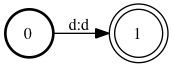
\includegraphics[scale=0.5]{images/d.jpg}
\end{center}

\noindent
Interpretation of the regular expression \texttt{dog} starts
with the building of simple networks for \texttt{d}, \texttt{o} and \texttt{g}, and
them combining them via the Concat() algorithm.  Interpretation of the entire regular expression
may involve creating many basic networks, combining them step by step into
successively
``larger''\footnote{The networks might not, of course, actually get larger.} networks via many calls to Concat(), Union(), Intersect(), Closure() and other
functions.  These operations usually introduce epsilon arcs, new states, and
non-determinism that can, in many instances, be eliminated via calls to
Determinize(), Minimize() and RmEpsilon().

The purpose of this paper is to explore how and when Determinize(), Minimize() and
RmEpsilon() can be invoked automatically during the interpretation of a regular
expression.

\section{Preliminaries}

The following statements reflect my understanding, and I'd be most grateful for
corrections:

\begin{enumerate}

\item
I will distinguish between theoretical/mathematical determinization
and the Determinize() algorithm provided in OpenFst.  The current Determinize()
algorithm in OpenFst has limitations that do not hold for
theoretical/mathe\-matical
determinization.  I will therefore distinguish between
\emph{determinize} and
\emph{Determinize()}, between \emph{determinization} and
\emph{Determinize()ation}, between \emph{determinized}
and \emph{Determinize()d}, etc.

\item
In particular, the current Determinize() algorithm requires that the argument network be
\emph{functional}.\footnote{Definition of Functional: for every input string, there is a single output
string.  The input string may match multiple paths in a transducer, but the output
must be the same for each path.}  Acceptors are always functional,
but transducers may be functional or non-functional.
Unfortunately, there is no easy or readily-available algorithm at
this time for testing functionality.

\item
We are informed by the OpenFst team that a future version of Determinize()
will not be restricted to functional networks.

\item
The Determinize() algorithm is intended, where possible, to determinize the 
\emph{input}
side of a transducer.  This is called input-side \emph{sequentialization} in some traditions.

\item
The current OpenFst Determinize() algorithm is written to treat weighted acceptors as basic.  (This, at least, is
what I understood from Johan Schalkwyk.)  

\item
The Determinize() algorithm is the  
algorithm described by Mohri in his 1997 Computational Linguistic
paper.\footnote{\emph{Finite-State Transducers in Language and Speech Processing}}
In the weighted automaton (i.e.\@ weighted acceptor) case, the implementation follows exactly  
Mohri's paper. A weighted transducer is dealt by considering the
weighted transducer over semiring K as the weighted automaton over the  
semiring obtained by taking the cross product of the string semiring  
and the semiring K. (From Cyril Allauzen, 13 Nov 2008.)

\item
The Encode() algorithm can be used to reduce transducers to
weighted acceptors so that they can be operated on safely by the
current Determinize() algorithm.

\item
Some networks cannot be determinized (a theoretical/mathematical limitation) because
the algorithm will never terminate. 

\begin{enumerate}
\item
Unweighted \emph{acceptors} can always be determinized and Determinize()d.

\item
If a transducer or acceptor is acyclic (no loops), it can always be determinized, but it may
not always be Determinize()d (using the current OpenFst Determinize() algorithm)
because
the current Determinize() algorithm has the additional requirement that the network be functional. 

\item
Determinization may not terminate for transducers and for weighted acceptors.
(MarkusD - 20 Jan 2009) ``[T]he determinization algorithm does  
not halt for certain weighted finite-state machines. This is described  
in Mohri 2004.\footnote{\url{http://www.cs.nyu.edu/~mohri/postscript/fla.pdf}} If  
the machine contains `sibling states' then they must be `twins'.  
Otherwise, the machine is not determinizable (under the commonly used  
semirings). Roughly, two states are sibling states if they are reachable from the  
start state on different paths that have the same label sequence, and  
there are cycles at these two states that have similar labels. If  
these two cycles have the same weight then they are twins.

On this machine,\footnote{MarkusD's example is shown in AT\&T text format for
acceptors, where each line indicates the SourceState, DestinationState, ArcLabel
and Weight.} for example, fstdeterminize doesn't terminate:

\begin{Verbatim}[fontsize=\small]
0 1 1 1
0 2 1 2
1 1 2 3
1 3 3 5
2 2 2 4
2 3 4 6
3
\end{Verbatim}

\item
To be Determinize()d, a transducer must be both acyclic and functional.

\item
There is, as far as I know, no easy way in OpenFst to test if a network is
functional.

\end{enumerate}


\item
But many networks that cannot be determinized
can still be Determinize()d if they are properly Encode()d first.  The result may
not be mathematically determinized, but the number of states and arcs may still be
reduced.

\item
A network must be determinized before it can be minimized.  A network must be
Determinize()d before it can be Minimize()d.

\end{enumerate}

\section{Encode() and Decode()}

OpenFst offers the Encode() algorithm, which offers two interesting options for
optimization: encoding just the \emph{labels}, or encoding both \emph{labels and weights}. 

\subsection{Encode()ing Labels for Optimizing Acyclic Networks}

\subsubsection{The Code}

Recall that if a network is acyclic and functional, it can be Determinize()d; but
recall also that there is no available test in OpenFst for functionality.  So to
safely optimize acyclic networks, we can first ``Encode() the labels''.  This means
that each input:output label is reduced to a single integer, effectively reducing
the network to an acceptor (weighted or unweighted).  

To Encode() the labels, one first instantiates an EncodeMapper, specifying
kEncodeLabels thus:

\begin{Verbatim}[fontsize=\footnotesize]
EncodeMapper<Arc> encoder(kEncodeLabels, ENCODE) ;
\end{Verbatim}

\noindent
When fstp is a pointer to an acyclic FST, this EncodeMapper is then used in the following way:


\begin{Verbatim}[fontsize=\footnotesize]
EncodeMapper<Arc> encoder(kEncodeLabels, ENCODE) ;

// for Encode, pass a ptr to encoder
Encode(fstp, &encoder) ;

// determinize the network in place
*fstp = DeterminizeFst<Arc>(*fstp, 
             DeterminizeFstOptions<Arc>(CacheOptions(true, 0)));

Minimize(fstp) ;

// for Decode, pass the encoder itself (not a pointer)
Decode(fstp, encoder) ;
\end{Verbatim}

The idiom to determinize a network in place was kindly supplied by
Cyril Allauzen, and is used throughout this paper.  The
off-the-shelf Determinize() algorithm is non-destructive, creating
and returning a new network.

\subsubsection{Why Encode() Labels for Acyclic Networks?}

As explained by Cyril Allauzen, ``The library currently only supports the determinization of functional  
transducers (if two successful paths have the same input label, they  
need to also have the same output label). The reason for that is that  
we use the weighted automata [i.e.\@ weighted acceptor]
determinization algorithm [i.e.\@ this is the current OpenFst
Determinize() algorithm], viewing the  
output labels as weights in the String semiring.

\subsubsection{Example}

Because the current Determinize() algorithm requires that any acylic
transducers to be Determinize()d also be
functional, it crashes if you try to Determinize() even the following trivial network:

\begin{center}
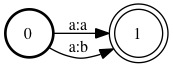
\includegraphics[scale=0.5]{images/aab.jpg}
\end{center}

\noindent
This example is not functional because the input string ``a'' has two outputs,
``a'' and ``b''.  After the labels are Encode()d, label \texttt{a:a} is reduced to
one integer, and label \texttt{a:b} is reduced to a different integer, and the
Determinize() algorithm runs on the functional result.  After Encode()ing the
labels, the result is an acceptor, and acceptors are always functional.

After the network is Decode()d, note that the result is not really
determinized in the mathematical sense at
all.  But this encoding-the-labels trick can still help to optimize many acyclic
networks, reducing the number of states and arcs.

\subsection{Encode()ing Labels and Weights}

In the previous subsection, we looked at \emph{a}cyclic networks and optimization;
now we're going to look at \emph{cyclic} networks and optimization.

If a network is \emph{cyclic} and, in addition, the semiring is idempotent, then it can still be Determinize()d
if you first Encode() both the labels \emph{and} the weights.  This reduces the network to an
unweighted acceptor, with each input:output/weight triple reduced to a single
integer. 

\subsubsection{The Code}

The code to Encode() both labels and weights looks like this:


\begin{Verbatim}[fontsize=\footnotesize]
EncodeMapper<Arc> encoder(kEncodeLabels | kEncodeWeights, ENCODE) ;

// for Encode, pass a ptr to encoder
Encode(fstp, &encoder) ;

// determinize in place
*fstp = DeterminizeFst<Arc>(*fstp, 
             DeterminizeFstOptions<Arc>(CacheOptions(true, 0)));

Minimize(fstp) ;

// for Decode, pass the encoder itself (not a pointer)
Decode(fstp, encoder) ;
\end{Verbatim}

\subsubsection{Why Encode() Labels \emph{and} Weights for Cyclic Networks?}

In general, you can't safely determinize cyclic networks, but Encode()ing the labels and
weights reduces the network to an unweighted acceptor, which is always
determinizable and Determinize()able.

The mathematical restriction (explained to me by Andr\'e Kempe) is that this
encode-labels-and-weights trick is valid only
for networks under \emph{idempotent} semirings, which include the
	Tropical Semiring.  (The Tropical Semiring is the
	standard/default semiring in OpenFst, and Kleene is currently
	limited to the Tropical Semiring.)
	Recall that an idempotent semiring has that property that for any weight w,
	Plus(w, w) = w.  In the Tropical Semiring, the Plus() operation is min(), and
	obviously min(w, w) = w.

The following example network highlights the restriction.  

\begin{center}
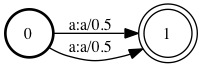
\includegraphics[scale=0.5]{images/cyclic.jpg}
\end{center}

\noindent
The start state
has two output arcs with the same label and the same weight.  When Encode() is
invoked for both labels and weights, the two arcs will have exactly the same
single-integer label.  Then when Determinize() is invoked, the sameness of the two arcs
will be recognized, and the two arcs will be conflated to one.  After decoding, the
original input:output labels and weight will be restored.  However, when two arcs
are conflated in this way, the weight should be the Plus() of the two original
weights.  For idempotent semirings, the original weight on both arcs (here 0.5) is the
appropriate result weight; but if the Plus() operation were simple addition, for
example, the decoded
result would have an incorrect weight.


\section{Determinize() and Minimize() Twice}

The Determinize() and Minimize() algorithms treat the epsilon as a normal symbol.

Cyril Allauzen has pointed out that the complexity of RmEpsilon() is quadratic, so
you want to reduce the size of a machine first using Determinize() and Minimize()
before invoking RmEpsilon(); and then call Determinize() and Minimize() again.
Thus, as a general rule, one would want to do the following
(pseudo-code):

\begin{Verbatim}[fontsize=\footnotesize]
Determinize()
Minimize()

if (!isEpsilonFree()) {
	RmEpsilon()

	Determinize()
	Minimize()
}
\end{Verbatim}

\section{An Algorithm for Optimization}

As best I understand things, the general algorithm for
mathematically-safe\footnote{Again, I understand that networks can blow up in size,
or require an inordinate amount of processing time, overwhelming your computer even
if the operations are mathematically safe.  Kleene will have to provide some way to
	turn off automatic optimization for cases that blow up.} optimization should be the
following:

\begin{Verbatim}[fontsize=\footnotesize]
if (isUnweighted(fstp) && isAcceptor(fstp)) {
    // no need to Encode
    // unweighed acceptors can always be determinized and Determinize()d

    // determinize in place
    *fstp = DeterminizeFst<Arc>(*fstp, 
                 DeterminizeFstOptions<Arc>(CacheOptions(true, 0)));
    Minimize(fstp) ;

    if (!isEpsilonFree(fstp)) {
	    RmEpsilon(fstp)

	    *fstp = DeterminizeFst<Arc>(*fstp, 
                 DeterminizeFstOptions<Arc>(CacheOptions(true, 0)));
    	Minimize(fstp) ;
	}
} elsif (isAcyclic(fstp)) {
    // any acyclic network can be determinized,
    // however, to Determinize() a network, using the current OpenFst
    // Determinize() algorithm, it must also be Functional.
    // To get around this restriction (and avoid crashes), 
    // Encode() the labels, reducing the network to an acceptor (which
    // is always functional)

    EncodeMapper<Arc> encoder(kEncodeLabels, ENCODE) ;

    Encode(fstp, &encoder) ;
    *fstp = DeterminizeFst<Arc>(*fstp, 
                 DeterminizeFstOptions<Arc>(CacheOptions(true, 0)));
    Minimize(fstp) ;
    Decode(fstp, encoder) ;

    if (!isEpsilonFree(fstp)) {
	    RmEpsilon(fstp) ;

    	Encode(fstp, &encoder) ;
    	*fstp = DeterminizeFst<Arc>(*fstp, 
                 DeterminizeFstOptions<Arc>(CacheOptions(true, 0)));
    	Minimize(fstp) ;
    	Decode(fstp, encoder) ;
	}
} elsif (isIdempotent(fstp)) { 
    // The network is cyclic
    // and the semiring is idempotent, then encode both labels and weights.
	// The semiring of the FST can be tested in C++ using
	// fstp->Type(), e.g.
	// if (fstp->Type() == "standard")

    EncodeMapper<Arc> encoder(kEncodeLabels | kEncodeWeights, ENCODE) ;

    Encode(fstp, &encoder) ;
    *fstp = DeterminizeFst<Arc>(*fstp, 
                 DeterminizeFstOptions<Arc>(CacheOptions(true, 0)));
    Minimize(fstp) ;
    Decode(fstp, encoder) ;

    if (!isEpsilonFree()) {
	    RmEpsilon(fstp) ;

    	Encode(fstp, &encoder) ;
    	*fstp = DeterminizeFst<Arc>(*fstp, 
                 DeterminizeFstOptions<Arc>(CacheOptions(true, 0)));
    	Minimize(fstp) ;
    	Decode(fstp, encoder) ;
	}
} else {
	RmEpsilon(fstp) ;
}
\end{Verbatim}

\noindent
The actual C++ code for this algorithm is called
\texttt{optimizeInPlace} and is found in \texttt{kleeneopenfst.cc},
which is the C++ bridge between Kleene (written in Java) and the
OpenFst library, which is written in C++.

\section{Still to be Resolved}

\begin{itemize}

\item
Kleene is currently limited to the default Tropical Semiring.
Generalizing it to handle multiple semirings will be a major
operation.\footnote{The Lextools family of programming languages,
built on the old AT\&T finite-state library by Richard Sproat, were
always limited to the default Tropical Semiring.}

\item
Is there a better way, other than \texttt{fstp->Type()}, to retrieve the semiring
or determine if the semiring of a network is idempotent?

\item
If a network is cyclic and not idempotent, it is always safe to call
RmEpsilon()?

\item
Other questions or problems?
\end{itemize}


\appendix
% causes subsequent sections to be lettered rather than numbered
%\section*{}  % to suppress lettering A, B, C of appendices

\section{Determinization and Minimization at PARC}

Some people reading this document will have experience with the Xerox/PARC Finite
State Toolkit.  
In the Xerox/PARC implementation, determinization and minimization are invoked
routinely on all intermediate and final networks, but this is possible only because 

\begin{itemize}
\item
The Xerox/PARC system handles only \emph{un}weighted networks, and

\item
Each arc label is stored as a single integer (which is a key into a separate table
that contains the separate input and output labels for transducers)

\item
The determinize and minimize operations see only the single integer label on each
arc

\end{itemize}

\noindent
Thus the Xerox/PARC networks lack weights, and the labels on arcs are like OpenFst
labels after the labels have been Encode()d.  As far as the Xerox/PARC determinize and
minimize algorithms are concerned, each network is always just an unweighted acceptor.

The corollary of this approach is that the Xerox/PARC implementation (at least the
publicly available one) doesn't offer input-side sequentialization (which is what
the OpenFst Determinize() is supposed to do).

\end{document}
